%%%%%%%%%%%%%%%%%%%%%%%%%%%%%%%%%%%%%%%%%%%%%%%%%%%%%%%%%%%%%%%%%%%%%%%%%%%%%%%%
\section{Recovering Dense 2D Correspondences: ``Face Flow''}\label{sec:face_flow_method}
%%%%%%%%%%%%%%%%%%%%%%%%%%%%%%%%%%%%%%%%%%%%%%%%%%%%%%%%%%%%%%%%%%%%%%%%%%%%%%%%
Let us assume that the input face video contains $F$ frames. Let $M\subset\R^2$
be a 2D domain that corresponds to the region of a mean face in neutral expression
that will be used as a template. We seek to estimate a function
$\bu(\bx;f) : M\times \{1,\ldots,F\} \rightarrow \R^2$ that represents the
optical flow from this domain to every frame of the input sequence.
More precisely, this function establishes the correspondence between every
facial point $\bx$ in the domain $M$ and its location at every frame index $f$,
which is given by the warping function $W_f(\bx)=\bx+\bu(\bx;f)$. This warping
function registers the $f$-th frame to the domain $M$.

Exploiting prior knowledge about the warping functions that are yielded from
facial deformations, we adopt a linear model for every $W_f(\bx)$ as follows:
%%%%%%%%%%%%%%%%%%%%%%%%%%%%%%%%%%%%%%%%%%%%%%%%%%%%%%%%%%%%%%%%%%%%%%%%%%%%%%%%
\begin{equation}
    W_f(\bx) = W(\bx;\bc_f) = \langle \bB(\bx) , \bc_f \rangle, \,\bx \in M,
\end{equation}
%%%%%%%%%%%%%%%%%%%%%%%%%%%%%%%%%%%%%%%%%%%%%%%%%%%%%%%%%%%%%%%%%%%%%%%%%%%%%%%%
where $\bB:M\rightarrow \R^{2 \times D}$ is a learnt basis of facial deformations that
contains $D$ basis vector elements and is common to all frames. Also,
$\bc_f\in\R^D$ is the coefficient vector for the $f$-th frame. $\bB(\bx)$ is 
constructed a priori during a training process and
therefore, for an input face video, we transform the multi-frame optical flow
estimation to the estimation of the following $D\times F$ matrix:
%%%%%%%%%%%%%%%%%%%%%%%%%%%%%%%%%%%%%%%%%%%%%%%%%%%%%%%%%%%%%%%%%%%%%%%%%%%%%%%%
\begin{equation}
    \matr{C} = \left[ \bc_1 \cdots \bc_f \cdots \bc_F \right] \,,
\end{equation}
%%%%%%%%%%%%%%%%%%%%%%%%%%%%%%%%%%%%%%%%%%%%%%%%%%%%%%%%%%%%%%%%%%%%%%%%%%%%%%%%
The $f$-th column of this matrix contains the coefficients that yield the
warping function (and thus define the optical flow) for the $f$-th frame of the
video. Following AAMs~\cite{cootes2001active}, the first 4 components of these coefficients, 
which correspond to the first 4 rows of the coefficient matrix $\matr{C}$, 
control the similarity transformation that rigidly-aligns the template to every 
frame. The remaining components control the non-rigid deformations. 
Therefore, we decompose $\matr{C}$ into the following sub-matrices:
%%%%%%%%%%%%%%%%%%%%%%%%%%%%%%%%%%%%%%%%%%%%%%%%%%%%%%%%%%%%%%%%%%%%%%%%%%%%%%%%
\begin{equation}\label{E:C_DEC}
    \matr{C} =
        \left[
            \begin{array}{l}
                \matr{C}_s\\
                \matr{C}_{nr} 
            \end{array}
        \right],
\end{equation}
%%%%%%%%%%%%%%%%%%%%%%%%%%%%%%%%%%%%%%%%%%%%%%%%%%%%%%%%%%%%%%%%%%%%%%%%%%%%%%%%
where $\matr{C}_s$ and $\matr{C}_{nr}$ correspond to the similarity and non-rigid 
part of the facial deformations respectively. 
$\matr{C}_s$ is a $4\times F$ matrix and $\matr{C}_{nr}$ is a $K \times F$ matrix, 
where $K=D-4$ is the rank of non-rigid deformations of the model.
%%%%%%%%%%%%%%%%%%%%%%%%%%%%%%%%%%%%%%%%%%%%%%%%%%%%%%%%%%%%%%%%%%%%%%%%%%%%%%%%
\section{Proposed Energy}
%%%%%%%%%%%%%%%%%%%%%%%%%%%%%%%%%%%%%%%%%%%%%%%%%%%%%%%%%%%%%%%%%%%%%%%%%%%%%%%%
Let $\bI(\bx;f):\Omega\times \{1,\ldots,F\} \rightarrow \R^{N_c}$ be the
$N_c$-channel sequence of frames of the input video, where $\Omega$ is the
rectangular image domain that corresponds to this video. The channels of the
input frames originate from the application of some appropriate feature descriptor.

As a preprocessing step, a frame of the sequence which is as close as possible to
a frontal pose and a neutral expression is selected as reference. This frame is
warped to the template domain $M$ in order to match a mean face. This selection
and warping estimation can be easily done automatically by fitting the face
with an automatic facial alignment method~\cite{kazemi2014one,matthews2004active}. 
In this case, we assume that there is a known correspondence between the sparse points
found by the alignment method and the reference frame of our basis. Once the
sparse landmarks have been acquired, it is simple to warp the image into the
reference frame using a warping function such as a thin-plate spline. This
procedure is identical to the one performed when building Active Appearance
Models, with the exception of only being performed on a single template image.
In short, this warped reference frame defines the template image 
$\bT(\bx):M \rightarrow \R^{N_c}$.

We also consider the case where, as further preprocessing, a sparse set of facial
landmarks is localised and tracked in the video. Let $L$ be the total number of
landmarks and $\bell_{i,f}\in\R^2$ the position of the $i$-th landmark on the
$f$-th frame. In addition, let $\hat{\bell}_i\in\R^2$ be the position of the
$i$-th landmark on the template image, which is computed by applying the warping
function on the corresponding landmark of the reference frame.

We propose to estimate the face flow through the minimisation of the following energy:
%%%%%%%%%%%%%%%%%%%%%%%%%%%%%%%%%%%%%%%%%%%%%%%%%%%%%%%%%%%%%%%%%%%%%%%%%%%%%%%%
\begin{equation}
    E(\matr{C}) = E_{img}(\matr{C}) + \beta E_{land}(\matr{C}) \,,
\end{equation}
%%%%%%%%%%%%%%%%%%%%%%%%%%%%%%%%%%%%%%%%%%%%%%%%%%%%%%%%%%%%%%%%%%%%%%%%%%%%%%%%
under the low-rank constraint:
%%%%%%%%%%%%%%%%%%%%%%%%%%%%%%%%%%%%%%%%%%%%%%%%%%%%%%%%%%%%%%%%%%%%%%%%%%%%%%%%
\begin{equation}\label{eq:lowrank}
    \mbox{rank}(\matr{C}_{nr}) \leq \lambda,
\end{equation}
%%%%%%%%%%%%%%%%%%%%%%%%%%%%%%%%%%%%%%%%%%%%%%%%%%%%%%%%%%%%%%%%%%%%%%%%%%%%%%%%
where $\matr{C}_{nr}$ is the non-rigid part of $\matr{C}$ in~\cref{E:C_DEC}. 
$E_{img}$ is an image data 
term and $E_{land}$ is a landmark term. The positive weight $\beta$ 
controls the balance between these terms, whereas the integer $0\leq\lambda\leq K$ is the 
imposed maximum rank of non-rigid deformations for the input sequence. 
We now define and explain the different parts of this minimisation problem.

The first term ($E_{img}$) enforces consistency of the feature descriptor values
of every point of the template over all frames:
%%%%%%%%%%%%%%%%%%%%%%%%%%%%%%%%%%%%%%%%%%%%%%%%%%%%%%%%%%%%%%%%%%%%%%%%%%%%%%%%
\begin{equation}\label{eq:eimg}
    E_{img} = \sum_{f=1}^F \int_M  \norm{
                \bT(\bx) -
               \bI\left( W(\bx;\bc_f) \,;\, f \right)
             }^2  \, \ud \bx,
\end{equation}
%%%%%%%%%%%%%%%%%%%%%%%%%%%%%%%%%%%%%%%%%%%%%%%%%%%%%%%%%%%%%%%%%%%%%%%%%%%%%%%%
In general, such an image data term could be grossly affected by artefacts in the 
image, such as illumination variation and external occlusions. Therefore, it is
common to use a robust penaliser rather than the quadratic term shown in 
\cref{eq:eimg}. However, we act on recent advancements in facial alignment 
algorithms~\cite{antonakos2015feature} that suggest that densely 
sampled feature descriptors can vastly improve the performance of alignment
algorithms without sacrificing the efficiency of a quadratic optimisation.
The use of dense descriptors is similar to SIFTFlow~\cite{liu2011sift}, where 
SIFT~\cite{lowe2004distinctive} features are densely sampled at every pixel in order
to improve optical flow.

The second term ($E_{land}$) is a quadratic prior that ensures that the estimated
face flow is in accordance with the landmark information on the corresponding
sparse points in every frame:
%%%%%%%%%%%%%%%%%%%%%%%%%%%%%%%%%%%%%%%%%%%%%%%%%%%%%%%%%%%%%%%%%%%%%%%%%%%%%%%%
\begin{equation}
    E_{land} = \sum_{f=1}^F \sum_{i=1}^L \norm{
                    W(\hat{\bell}_i;\bc_f) - \bell_{i,f}
                }^2,
\end{equation}
%%%%%%%%%%%%%%%%%%%%%%%%%%%%%%%%%%%%%%%%%%%%%%%%%%%%%%%%%%%%%%%%%%%%%%%%%%%%%%%%
Regarding the low-rank constraint~\cref{eq:lowrank}, it is natural to assume that the deformations
of the face over time are highly correlated and thus lie in a low-dimensional subspace.
However, the similarity transformations describing the face motion are, in general, not 
sufficiently correlated with the non-rigid deformations that the face undergoes. For example,
the similarity transformations often originate from camera motion. Consequently, we penalise the number of 
independent components needed to describe the non-rigid face deformations of the specific input 
sequence and thus impose $\matr{C}_{nr}$ to be of low-rank.
%%%%%%%%%%%%%%%%%%%%%%%%%%%%%%%%%%%%%%%%%%%%%%%%%%%%%%%%%%%%%%%%%%%%%%%%%%%%%%%%
\subsection{Estimation of the Sparse Landmarks}
%%%%%%%%%%%%%%%%%%%%%%%%%%%%%%%%%%%%%%%%%%%%%%%%%%%%%%%%%%%%%%%%%%%%%%%%%%%%%%%%
In order to estimate sparse landmarks, we can make use of state-of-the-art, extremely
efficient facial alignment methods~\cite{kazemi2014one,asthana2014incremental,%
menpo14,alabort2014bayesian}.
State-of-the-art methods, such as that by \citet{kazemi2014one},
execute in under a millisecond, and can provide landmark localisation errors
of within $3$ pixels on average for extremely challenging unconstrained images.
In this chapter, when we consider estimating landmarks, we use the method of 
\citet{kazemi2014one} in conjunction with a robust face detector~\cite{zafeiriou2015survey}.
%%%%%%%%%%%%%%%%%%%%%%%%%%%%%%%%%%%%%%%%%%%%%%%%%%%%%%%%%%%%%%%%%%%%%%%%%%%%%%%%
\section{Optimisation of the Proposed Energy}
%%%%%%%%%%%%%%%%%%%%%%%%%%%%%%%%%%%%%%%%%%%%%%%%%%%%%%%%%%%%%%%%%%%%%%%%%%%%%%%%
The image data term is highly non-convex, therefore we have to adopt an iterative
linearisation scheme. For this scheme to be computationally efficient, we consider
an inverse compositional (IC) strategy. In every iteration, we seek to update the
current estimate $\matr{\tilde{C}}= [\tilde{\bc}_1 \cdots \tilde{\bc}_F]$ of the
coefficient matrix. In addition, we consider a spatial discretisation of $E_{img}$ 
on a regular pixel grid with unary steps. Let $\bx_1,\ldots,\bx_P$ be the 2D 
locations of the $P$ pixels that lie within the domain $M$.

The IC algorithm, as proposed by~\cite{baker2004lucas}, is a very efficient method of solving
a parametrised image alignment problem, which corresponds to minimising solely the image data 
term $E_{img}$ of the proposed energy for every frame of the sequence. Given a single 
template image $\bT$ and a single input image $\bI$, the classical 
Lucas-Kanade~\cite{lucas1981iterative} problem is given by
%%%%%%%%%%%%%%%%%%%%%%%%%%%%%%%%%%%%%%%%%%%%%%%%%%%%%%%%%%%%%%%%%%%%%%%%%%%%%%%%
\begin{equation}\label{eq:lk_ic}
    \sum_{p=1}^P  \norm{
                         \bT(W(\bx_p;\Delta \bc)) -
                         \bI\left( W(\bx_p;\bc) \right)
                        }^2,
\end{equation}
%%%%%%%%%%%%%%%%%%%%%%%%%%%%%%%%%%%%%%%%%%%%%%%%%%%%%%%%%%%%%%%%%%%%%%%%%%%%%%%%
which is minimised for $\Delta \bc$, the parameters of the warp for a single image. 
Here, $\bT(W(\bx_p;\Delta \bc))$ denotes 
the template warped around the current linearised estimate of $\Delta \bc$.
The IC algorithm is so efficient because we assume that we
linearise \cref{eq:lk_ic} around $\Delta \bc$ and thus the template
is fixed and does not require warping during the updates. To update the parameters
$\bc$, a compositional update is performed: 
$W(\bx_p;\Delta \bc) \leftarrow W(\bx_p;\Delta \bc) \cdot {W(\bx_p;\Delta \bc)}^{-1}$.
This update ensures that the derivative with respect to the warp is also fixed
and therefore we arrive at the extremely efficient update for $\bc$:
%%%%%%%%%%%%%%%%%%%%%%%%%%%%%%%%%%%%%%%%%%%%%%%%%%%%%%%%%%%%%%%%%%%%%%%%%%%%%%%%
\begin{equation}\label{eq:lk_ic_update}
    \Delta \bc = {(\bJ^T \bJ)}^{-1} \sum_{p=1}^P \bJ^T [\bI\left( W(\bx_p;\bc) \right) - \bT(\bx_p)],
\end{equation}
%%%%%%%%%%%%%%%%%%%%%%%%%%%%%%%%%%%%%%%%%%%%%%%%%%%%%%%%%%%%%%%%%%%%%%%%%%%%%%%%
where $\bJ = \nabla \bT \frac{\partial W}{\partial \bc}$,
and the derivative $\frac{\partial W}{\partial \bc}$ is 
taken around $(\bx_p;\boldsymbol{0}) = \bB(\bx_p)$. Therefore,
the entire Hessian term $\boldsymbol{H} = \bJ^T \bJ$, does not depend
on $\bc$ and can be precomputed.
Unlike in most previous works in the area, our motion model is completely 
translational and thus does not involve a complicated compositional update. 
In fact, it can be shown that our compositional update
has the form $\bc \leftarrow \bc - \Delta \bc$ and is thus equivalent to the 
additive parameter update scheme~\cite{amberg2009compositional}.

Returning to the optimisation of the proposed energy, the
image data term can be approximated as (after the IC strategy and the spatial
discretisation):
%%%%%%%%%%%%%%%%%%%%%%%%%%%%%%%%%%%%%%%%%%%%%%%%%%%%%%%%%%%%%%%%%%%%%%%%%%%%%%%%
\begin{equation}
    E_{img} \approx \sum_{f=1}^F \sum_{p=1}^P  \norm{
                                    \bT(W(\bx_p;\Delta \bc_f)) -
                                   \bI\left( W(\bx_p;\tilde{\bc}_f)\,;\, f \right)
                                 }^2,
\end{equation}
%%%%%%%%%%%%%%%%%%%%%%%%%%%%%%%%%%%%%%%%%%%%%%%%%%%%%%%%%%%%%%%%%%%%%%%%%%%%%%%%
where $\Delta \bc_f$ are the additive warp parameters for frame $f$. 
Note that $\Delta \bc_f = \bc_f - \tilde{\bc}_f$, a relation that we use since
in our formulation, in contrast to the traditional IC algorithm, we incorporate
terms that depend directly on $\bc_f$.
By considering linearisations of the template in the above equation and rewriting
the terms using compact matrix notation over all pixels and frames, the total
proposed energy becomes:
%%%%%%%%%%%%%%%%%%%%%%%%%%%%%%%%%%%%%%%%%%%%%%%%%%%%%%%%%%%%%%%%%%%%%%%%%%%%%%%%
\begin{equation}\label{E:ENERGY}
    E(\matr{C}) \approx \norm{ \matr{R} + \matr{J} (\matr{C} - \matr{\tilde{C}}) }_F^2
    + \beta \norm{\matr{B}_\ell \matr{C} - \matr{L}_{loc}}_F^2,
\end{equation}
%%%%%%%%%%%%%%%%%%%%%%%%%%%%%%%%%%%%%%%%%%%%%%%%%%%%%%%%%%%%%%%%%%%%%%%%%%%%%%%%
where $\matr{R}$ is a $(P N_c) \times F$ matrix that contains the error residuals
$\bT(\bx_p) - \bI\left( W(\bx_p;\tilde{\bc}_f) \,;\, f \right)$ for all pixels
$p$ and frames $f$. Also,
$\matr{J}$ is a $(P N_c) \times D$ matrix that contains the template Jacobian
$\nabla\bT(\bx_p) \bB(\bx_p)$ for all pixels.
Finally, $\matr{B}_\ell$ is a $2L \times D$ matrix consisting of the deformation
basis evaluated at the locations of the landmarks on the template and
$\matr{L}_{loc}$ is a $2L\times F$ matrix with the coordinates of the landmarks
in all frames:
%%%%%%%%%%%%%%%%%%%%%%%%%%%%%%%%%%%%%%%%%%%%%%%%%%%%%%%%%%%%%%%%%%%%%%%%%%%%%%%%
\begin{equation}
    \matr{B}_\ell=
        \left[
            \begin{array}{c}
                \bB(\hat{\bell}_1) \\
                \vdots \\
                \bB(\hat{\bell}_L)
            \end{array}
        \right],\,
    \matr{L}_{loc}=
        \left[
            \begin{array}{ccc}
                \bell_{1,1}&\cdots&\bell_{1,F}
                \\
                \vdots&&\vdots
                \\
                \bell_{L,1}&\cdots&\bell_{L,F}
            \end{array}
        \right],
\end{equation}
%%%%%%%%%%%%%%%%%%%%%%%%%%%%%%%%%%%%%%%%%%%%%%%%%%%%%%%%%%%%%%%%%%%%%%%%%%%%%%%% 

Using the decomposition of $\matr{C}$ in a similarity and a
non-rigid part (\cref{E:C_DEC}), the energy of \cref{E:ENERGY} is written as:
%%%%%%%%%%%%%%%%%%%%%%%%%%%%%%%%%%%%%%%%%%%%%%%%%%%%%%%%%%%%%%%%%%%%%%%%%%%%%%%% 
\begin{eqnarray*}%\label{E:ENERGY_PARTS}
    &&E(\matr{C}_s,  \matr{C}_{nr} ) \approx \\
    &    &\norm{ \matr{R} + \matr{J}_{nr} (\matr{C}_{nr} - \matr{\tilde{C}}_{nr}) + \matr{J}_{s} (\matr{C}_{s} - \matr{\tilde{C}}_{s}) }_F^2 \nonumber \\
    &     &+ \beta \norm{{\matr{B}_\ell}_{nr} \matr{C}_{nr} - {\matr{B}_\ell}_{s} \matr{C}_{s} - \matr{L}_{loc}}_F^2,
\end{eqnarray*}
%%%%%%%%%%%%%%%%%%%%%%%%%%%%%%%%%%%%%%%%%%%%%%%%%%%%%%%%%%%%%%%%%%%%%%%%%%%%%%%% 
Consequently, we propose to solve the following rank constraint optimisation problem:
%%%%%%%%%%%%%%%%%%%%%%%%%%%%%%%%%%%%%%%%%%%%%%%%%%%%%%%%%%%%%%%%%%%%%%%%%%%%%%%% 
\begin{equation}\label{E:MINIMIZATION}
    \min_{\matr{C}_s,  \matr{C}_{nr}} E(\matr{C}_s,  \matr{C}_{nr} ) \quad \mbox{s.t.} \quad \mbox{rank}(\matr{C}_{nr}) \leq \lambda,
\end{equation}
%%%%%%%%%%%%%%%%%%%%%%%%%%%%%%%%%%%%%%%%%%%%%%%%%%%%%%%%%%%%%%%%%%%%%%%%%%%%%%%% 
Although \cref{E:MINIMIZATION} is a non-convex problem, it can be solved efficiently
by employing a block-coordinate descent (BCD) scheme. Let $t$ be the iteration index. The 
iteration of BCD for \cref{E:MINIMIZATION} reads as follows:
%%%%%%%%%%%%%%%%%%%%%%%%%%%%%%%%%%%%%%%%%%%%%%%%%%%%%%%%%%%%%%%%%%%%%%%%%%%%%%%% 
\begin{eqnarray}
    & &\matr{C}_s[t+1] =  \min_{\matr{C}_s[t]} E(\matr{C}_s[t],  \matr{C}_{nr}[t] ), \label{E:SUB1} \\ 
    & & \matr{C}_{nr}[t+1] =  \min_{\matr{C}_{nr}[t+1]} E(\matr{C}_s[t+1],  \matr{C}_{nr}[t] ), \nonumber \\
    & &\quad \mbox{s.t.} \quad \mbox{rank}(\matr{C}_{nr}) \leq \lambda. \label{E:SUB2}
\end{eqnarray}
%%%%%%%%%%%%%%%%%%%%%%%%%%%%%%%%%%%%%%%%%%%%%%%%%%%%%%%%%%%%%%%%%%%%%%%%%%%%%%%% 
The sub-problem \cref{E:SUB1} is a least-squares problem admitting a closed-form solution. 

The sub-problem \cref{E:SUB2} is also solved in closed-form. First, let us define the matrices
%%%%%%%%%%%%%%%%%%%%%%%%%%%%%%%%%%%%%%%%%%%%%%%%%%%%%%%%%%%%%%%%%%%%%%%%%%%%%%%% 
\begin{equation}\label{E:Mat}
    \matr{A}=
        \left[
            \begin{array}{l}
               \matr{R} + \matr{J}_{s} (\matr{C}_{s} - \matr{\tilde{C}}_{s}) \\
               {\matr{B}_\ell}_{s} \matr{C}_{s} - \matr{L}_{loc}
            \end{array}
        \right],\,
    \matr{Q}=
        \left[
            \begin{array}{l}
                \matr{J}_{nr} \\
                {\matr{B}_{\ell}}_{nr}
            \end{array}
        \right],
\end{equation}
%%%%%%%%%%%%%%%%%%%%%%%%%%%%%%%%%%%%%%%%%%%%%%%%%%%%%%%%%%%%%%%%%%%%%%%%%%%%%%%% 
with $\matr{Q} = \matr{U}\matr{\Sigma}\matr{V}$ being the 
Thin Singular Value Decomposition of $\matr{Q}$,
$\matr{Q}^{\dag}$ denoting the pseudo-inverse of $\matr{Q}$,
$\matr{\Xi} = \matr{U}\matr{U}^T\matr{A}$, and $\matr{\Xi}_{(\lambda)}$ being the 
$\lambda$-rank approximation of $\matr{\Xi}$.
Then by using \cref{E:Mat},  \cref{E:SUB2} is written as:
%%%%%%%%%%%%%%%%%%%%%%%%%%%%%%%%%%%%%%%%%%%%%%%%%%%%%%%%%%%%%%%%%%%%%%%%%%%%%%%% 
\begin{equation}\label{E:RedRank}
    \min_{\matr{C}_{nr}} \norm{\matr{A}  - \matr{Q} \matr{C}_{nr}}_F^2 \quad \mbox{s.t.} \quad  \mbox{rank}(\matr{C}_{nr}) \leq \lambda,
\end{equation}
%%%%%%%%%%%%%%%%%%%%%%%%%%%%%%%%%%%%%%%%%%%%%%%%%%%%%%%%%%%%%%%%%%%%%%%%%%%%%%%% 
The closed form solution of \cref{E:RedRank} is given by~\cite{sondermann1986best}: 
%%%%%%%%%%%%%%%%%%%%%%%%%%%%%%%%%%%%%%%%%%%%%%%%%%%%%%%%%%%%%%%%%%%%%%%%%%%%%%%% 
\begin{equation}
    \matr{C}_{nr}  = \matr{Q}^{\dag}\matr{\Xi}_{(\lambda)}  \,.
\end{equation}
%%%%%%%%%%%%%%%%%%%%%%%%%%%%%%%%%%%%%%%%%%%%%%%%%%%%%%%%%%%%%%%%%%%%%%%%%%%%%%%% 
The convergence of the proposed BCD algorithm is guaranteed since the objective function
is differentiable and involves two blocks of variables~\cite{luo1992convergence}.
%%%%%%%%%%%%%%%%%%%%%%%%%%%%%%%%%%%%%%%%%%%%%%%%%%%%%%%%%%%%%%%%%%%%%%%%%%%%%%%%
\section{Building a 2D Deformation Model}\label{sec:face_flow_learning_deformation}
%%%%%%%%%%%%%%%%%%%%%%%%%%%%%%%%%%%%%%%%%%%%%%%%%%%%%%%%%%%%%%%%%%%%%%%%%%%%%%%%
Learning the deformation basis is a very challenging issue and most likely the reason
why there is little existing research into building \textit{dense} 2D facial deformation models.
The primary difficulty in densifying the annotation sets available for faces
is the ambiguity inherent in labelling sub-pixel locations. This is particularly
challenging in low-texture areas such as the cheeks. For this reason, the 
existing databases for face alignment~\cite{sagonas2013300,zhu2012face,%
belhumeur2013localizing,le2012interactive} were all manually annotated with
different sets of \textit{sparse} feature points. 
Even the densest annotation set, that of HELEN~\cite{le2012interactive}, 
was semi-automatically annotated due to the difficulty of semantically
labelling only $194$ points. Therefore, it remains infeasible to manually
annotate the density of fiducial points required in this chapter. Thus, we
propose two methods of building a dense 2D facial deformation model based
on automatic data generation: using the output of optical flow methods and
rendering a 3D statistical model.

%%%%%%%%%%%%%%%%%%%%%%%%%%%%%%%%%%%%%%%%%%%%%%%%%%%%%%%%%%%%%%%%%%%%%%%%%%%%%%%%
\begin{figure}[t]
    \centering
    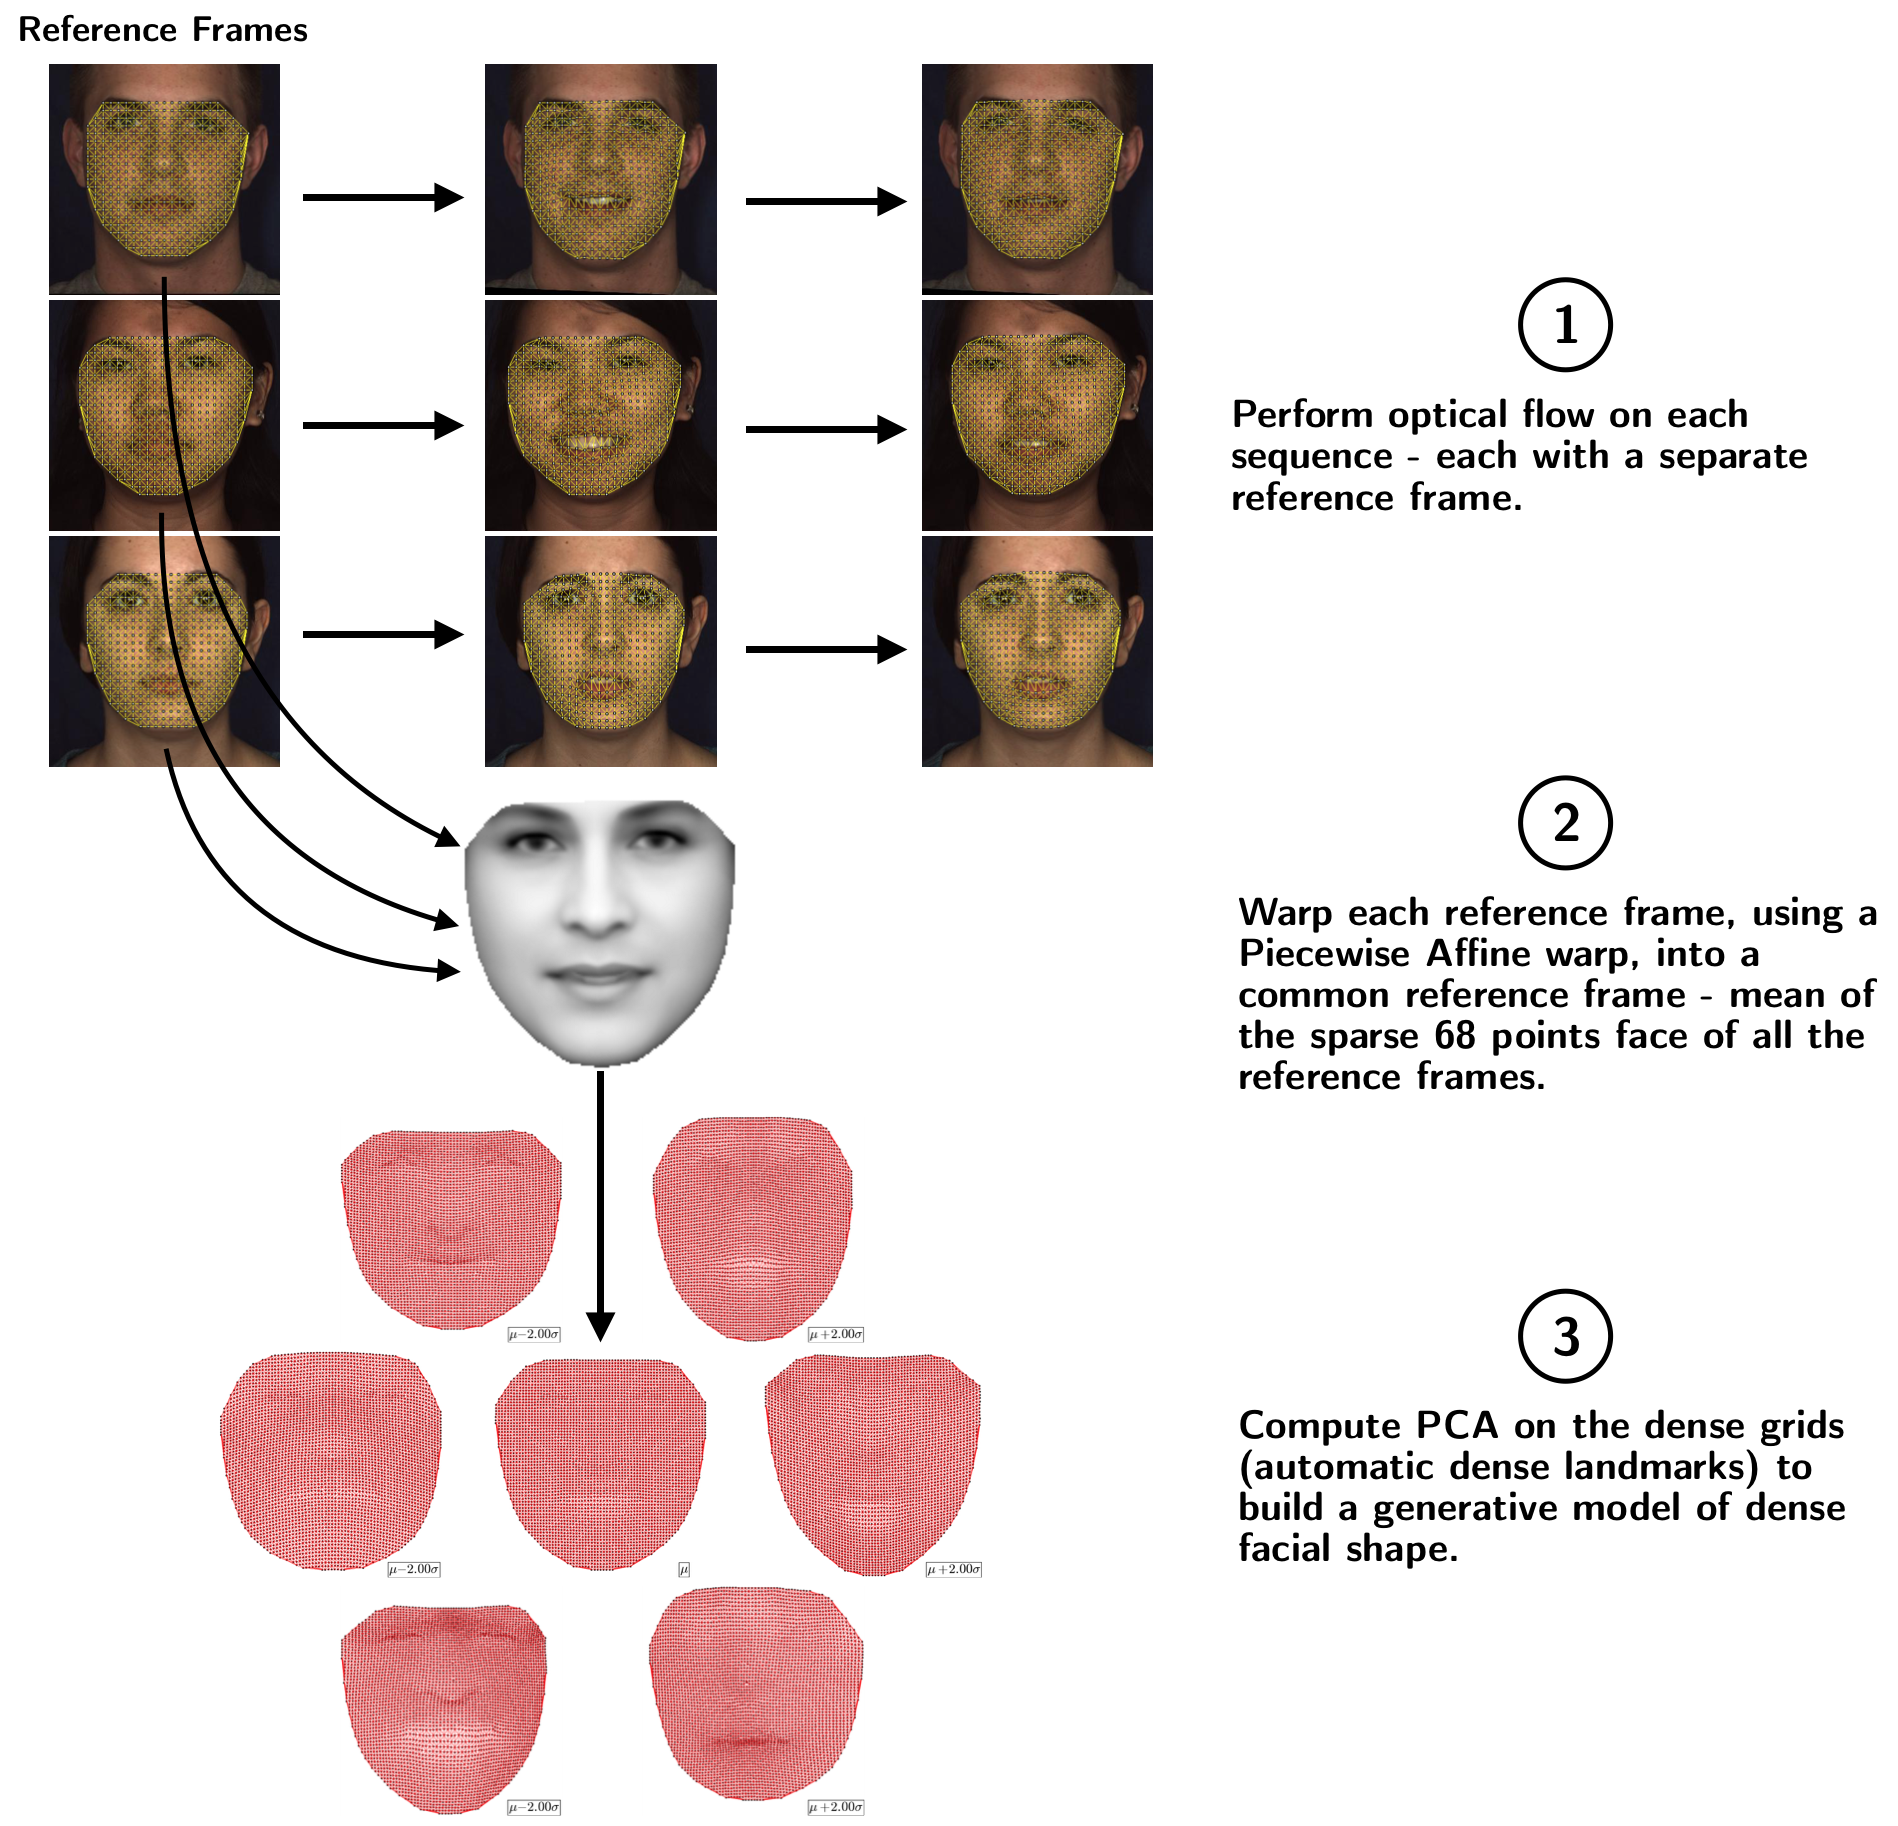
\includegraphics[width=\textwidth]{face_flow/images/of_pca_basis/optical_flow_basis_construction}
    \caption{A diagram of the optical flow construction strategy used in this
             Chapter.}
\label{fig:optical_flow_pca_basis_construction}
\end{figure}
%%%%%%%%%%%%%%%%%%%%%%%%%%%%%%%%%%%%%%%%%%%%%%%%%%%%%%%%%%%%%%%%%%%%%%%%%%%%%%%%
\textbf{Optical Flow.}
Inspired by the performance of recent optical methods on long, clean sequences,
we propose to train a statistical model on the output of these methods. 
Although computing these initial flows is costly, the learnt deformation model
allows us to efficiently approximate these deformations on more challenging
sequences. To realise this, we chose the optical flow method of
\citet{garg2013variational}, augmented with an additional quadratic penalty
to guide the flows towards automatically estimated sparse landmarks.
This additional penalty was found to significantly improve the performance
of~\cite{garg2013variational} in highly expressive sequences, such as those with 
large openings of the mouth.

We propose to learn a set of trajectories over a number of sequences, each with
a differing reference frame. We are thus faced with the problem
of achieving correspondence between these reference frames for the construction
of the deformation basis. Given that each frame contains estimated sparse landmarks,
we calculate the mean position of each landmark and define the area of spatial support
for our deformation basis, $M$, to be the pixels that are situated inside the
convex hull of these positions. Once the reference frame is constructed,
each set of trajectories is converted into endpoints for each frame, analogous
to dense landmarks for the image, and sampled into the reference frame using
a thin-plate splines warp parametrised by the automatically estimated landmarks.
Finally, given that we have a set of dense landmarks in correspondence, we perform a 
Procrustes alignment in order to normalise any scale issues that may be present.
%%%%%%%%%%%%%%%%%%%%%%%%%%%%%%%%%%%%%%%%%%%%%%%%%%%%%%%%%%%%%%%%%%%%%%%%%%%%%%%%
\begin{figure}
    \centering
    \hspace*{\fill}
    \begin{subfigure}[b]{0.125\textheight}
        \centering
        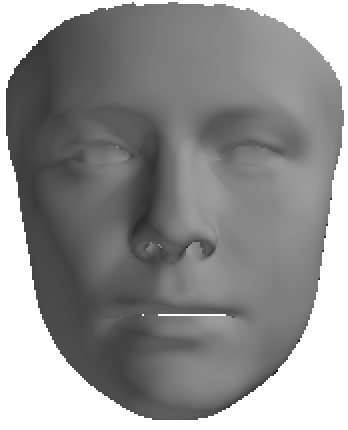
\includegraphics[width=\textwidth]{face_flow/images/contour_snapping/original_3d_model_mean}
        \caption{Mean}\label{subfig:face_flow_original_3d_mean}
    \end{subfigure} \hfill
    \begin{subfigure}[b]{0.23\textheight}
        \centering
        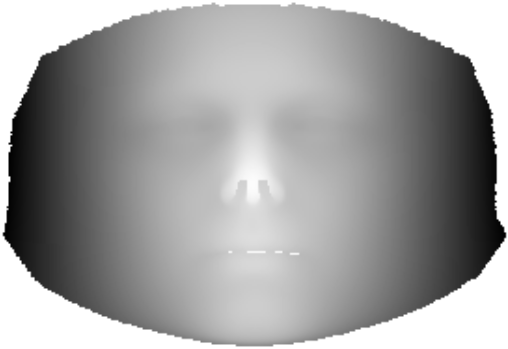
\includegraphics[width=\textwidth]{face_flow/images/contour_snapping/cylindrically_unwrapped}
        \caption{Cylindrically Unwrapped Mean}\label{subfig:face_flow_cylin_unwrap}
    \end{subfigure} \hfill
    \begin{subfigure}[b]{0.135\textheight}
        \centering
        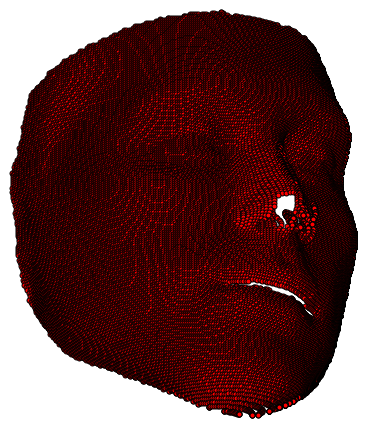
\includegraphics[width=\textwidth]{face_flow/images/contour_snapping/example_instance_high}
        \caption{High Resolution}\label{subfig:face_flow_instance_high}
    \end{subfigure} \hfill
    \begin{subfigure}[b]{0.13\textheight}
        \centering
        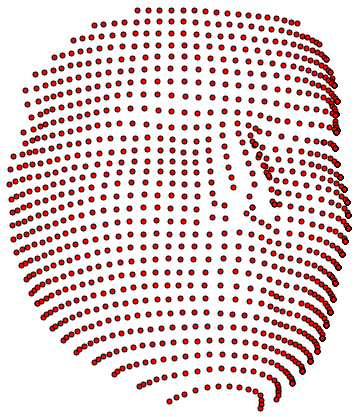
\includegraphics[width=\textwidth]{face_flow/images/contour_snapping/example_instance_low}
        \caption{Low resolution}\label{subfig:face_flow_instance_low}
    \end{subfigure}
    \hspace*{\fill}
    \caption{The model construction pipeline for the 2D deformation basis based
             on the 3D statistical model. Top row shows both the cylindrically 
             unwrapped 2D atlas and the original model mean in 3D. Bottom row
             shows a high and low resolution re-sampled instance of the rendered
             3D model.}
\label{fig:face_flow_3d_model_instance}
\end{figure}
%%%%%%%%%%%%%%%%%%%%%%%%%%%%%%%%%%%%%%%%%%%%%%%%%%%%%%%%%%%%%%%%%%%%%%%%%%%%%%%%

\textbf{3D Statistical Model.}
Although the 2D deformation basis learnt from optical flow yields a plausible
set of deformations for human faces, it does have a number of disadvantages.
Firstly, computing optical flow in the presence of large out-of-plane rotations,
such as the turning of a head, is a clear violation of the optical flow assumption
that a pixel is visible between two frames. For this reason, incorporating pose into the
sequences makes computing the initial flows accurately a difficult process.
Furthermore, even in the case where reasonable flow can be computed for a 
sequence containing head rotations\footnote{As shown by \citet{garg2013dense}},
computing correspondences between different sequences becomes challenging
as the piecewise warping procedure above does not generalise well across large
poses. This is in part due to the difficulty of estimating sparse landmarks
in the presence of large poses and the artefacts caused by the piecewise warping
procedure from non-frontal poses back to neutral.
To work around this, we propose to render an expressive 3D statistical model
under various expressions and poses and use the 2D projected positions
to describe our deformation basis. 

The main difficulty with using a 3D statistical model, such as that of
\citet{paysan20093d} or \citet{booth2016lsfm}, to construct a 2D
deformation basis is how to deal with self occlusions. These are not present when
building a model from optical flow as optical flow cannot model such 3D rotations.
These self-occlusions are an issue as when the face rotates around the yaw axis 
(left-right out-of-plane rotation) the far side of the face becomes occluded
by the near side. Naively projecting the 3D points causes the points on the far
side to become coincident with those on the nearside which will cause artefacts
when sampling pixels for the reference frame. An example of this issue
is given in \cref{fig:face_flow_pose_example} where it is shown that highly
salient regions such as the eye may be duplicated. This is a challenge for 
performing alignment as regions such as the eye provide strong texture cues and
thus these artefacts will heavily bias the recovered correspondences. To combat
this, we borrow from previous works that modify the projections to be more
consistent with the occluding contour~\cite{Zhu:2015ur,zhu2015high,hassner2015effective}.
Following \citet{zhu2015high} we assume the face to be approximately cylindrical and
cylindrically unwrap the face to construct a 2D atlas. The cylindrical unwrapping
of a point ${[x, y, z]}^T$ is given by the following mapping:
%%%%%%%%%%%%%%%%%%%
\begin{equation}
    \begin{aligned}
        \tilde{x} &\rightarrow r \theta \\
        \tilde{y} &\rightarrow y \\
        \tilde{z} &\rightarrow d
    \end{aligned}
\end{equation}
%%%%%%%%%%%%%%%%%%%
where $d = \sqrt{x^2 + y^2} - r$,
$\theta = \arctan{\left(\frac{x}{z}\right)}$ and $r$ is the provided radius 
specifying how wide the cyldinder is. Here we assume we discard the z
coordinate in order to yield a 2D atlas.
We then re-sample the mean mesh by rendering it into the area constructed by the
cylindrical unwrapping. An example of the cylindrically unwrapped atlas is given
in \cref{subfig:face_flow_cylin_unwrap}. 
This cylindrically unwrapped atlas has two functions: firstly it
allows simple construction of a multi-scale model by interpolating the vertices 
via rendering into the texture mapped region provided by the atlas. 
This is demonstrated by the high
and low resolution figures given in 
\cref{subfig:face_flow_instance_high,subfig:face_flow_instance_low}. Secondly,
it allows a simple method of snapping any vertices that are occluded back
onto the occluding contour. By first removing any in-plane rotation, the
visibility mask can be used to trace occluded pixels back to their nearest
non-occluded vertex position. For example, \cref{subfig:face_flow_snapped_contour}
shows where all the occluded vertices of \cref{subfig:face_flow_occluded_vis_mask}
are snapped to for the input image of \cref{subfig:face_flow_occluded_input}.
Note that \cref{subfig:face_flow_snapped_contour} has been rotated back
``upright'' to remove the in-plane rotation. The effect of this sampling can be seen in
\cref{subfig:face_flow_snapped_sampling} where we can see that the snapped
vertices are no longer coincident with the eye region. After the snapping of
occluded pixels back to the contour, the in-plane rotation can be reapplied
to recover the initial projection.
%%%%%%%%%%%%%%%%%%%%%%%%%%%%%%%%%%%%%%%%%%%%%%%%%%%%%%%%%%%%%%%%%%%%%%%%%%%%%%%%
\begin{figure}[t]
    \centering
    \hspace*{\fill}
    \begin{subfigure}[b]{0.2\textheight}
        \centering
        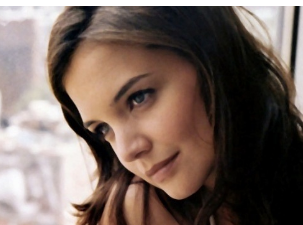
\includegraphics[width=\textwidth]{face_flow/images/contour_snapping/posed_head}
        \caption{Original Image~\cite{sagonas2013300}}\label{subfig:face_flow_occluded_input}
    \end{subfigure} \hfill
    \begin{subfigure}[b]{0.2\textheight}
        \centering
        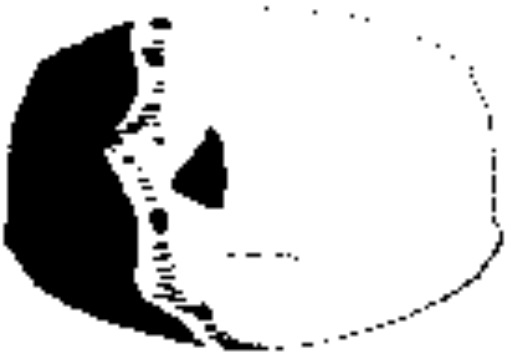
\includegraphics[width=\textwidth]{face_flow/images/contour_snapping/posed_visibility_mask}
        \caption{Visibility Mask}\label{subfig:face_flow_occluded_vis_mask}
    \end{subfigure} \hfill
    \begin{subfigure}[b]{0.2\textheight}
        \centering
        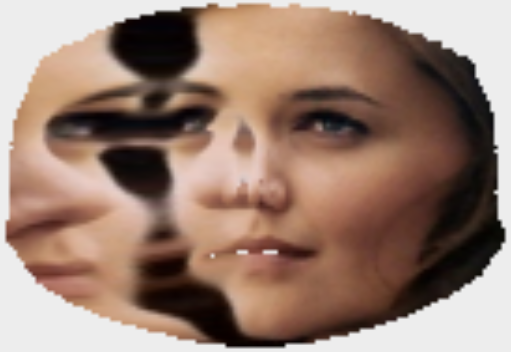
\includegraphics[width=\textwidth]{face_flow/images/contour_snapping/sampled_no_snapping}
        \caption{Naive Sampling}\label{subfig:face_flow_occluded_naive}
    \end{subfigure}
    \hspace*{\fill}
    \caption{An example of the effect the occluded points have on sampling the
             reference texture for the input in
             \cref{subfig:face_flow_occluded_input}. The visibility mask in
             \cref{subfig:face_flow_occluded_vis_mask} shows the occluded
             vertices as black and the naive sampling is shown in
             \cref{subfig:face_flow_occluded_naive}. Note how the eye is
             duplicated by the occluded points.}
\label{fig:face_flow_pose_example}
\end{figure}
%%%%%%%%%%%%%%%%%%%%%%%%%%%%%%%%%%%%%%%%%%%%%%%%%%%%%%%%%%%%%%%%%%%%%%%%%%%%%%%%

Given this new cylindrically unwrapped mesh we propose to sample
instances of the 3D statistical model, rotate them in 3D and then project them
into 2D using a weak perspective projection. As discussed, some vertices
will be occluded and these are snapped to the occluding contour. Finally, a
barycentric coordinate mapping from the original mesh to the cylindrically
unwrapped mesh is used in order to displace the mean vertices of the cylindrically
unwrapped mesh according to the instance of the 3D model. Many renderings of this
kind are produced and from these 2D shapes we construct a 2D deformation basis
that jointly describes pose, identity and expression. An example of such a basis
is given by \cref{fig:face_flow_3d_pca_basis}.
%%%%%%%%%%%%%%%%%%%%%%%%%%%%%%%%%%%%%%%%%%%%%%%%%%%%%%%%%%%%%%%%%%%%%%%%%%%%%%%%
\begin{figure}[t]
    \centering
    \hspace*{\fill}
    \begin{subfigure}[b]{0.23\textwidth}
        \centering
        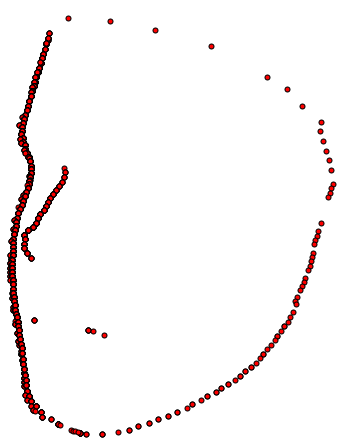
\includegraphics[width=\textwidth]{face_flow/images/contour_snapping/posed_snapped_contour}
        \caption{Snapped Vertices}\label{subfig:face_flow_snapped_contour}
    \end{subfigure} \hfill
    \begin{subfigure}[b]{0.4\textwidth}
        \centering
        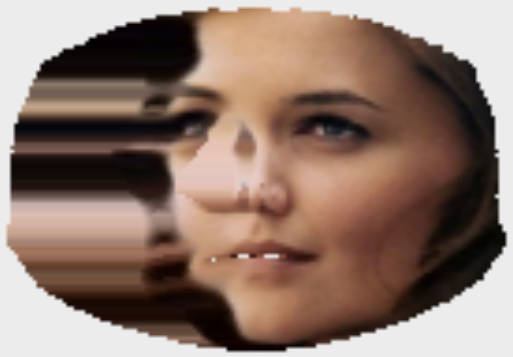
\includegraphics[width=\textwidth]{face_flow/images/contour_snapping/sampled_snapping}
        \caption{Occluded Contour Sampled}\label{subfig:face_flow_snapped_sampling}
    \end{subfigure}
    \hspace*{\fill}
    \caption{\cref{subfig:face_flow_snapped_contour} shows the vertices that
             been snapped to occluding contours. Note this includes areas such
             as the nose. \cref{subfig:face_flow_snapped_sampling} shows an
             example of sampling the texture of
             \cref{subfig:face_flow_occluded_input} with the occluding contour
             snapped mesh.}
\label{fig:face_flow_snapping_example}
\end{figure}
%%%%%%%%%%%%%%%%%%%%%%%%%%%%%%%%%%%%%%%%%%%%%%%%%%%%%%%%%%%%%%%%%%%%%%%%%%%%%%%%
%%%%%%%%%%%%%%%%%%%%%%%%%%%%%%%%%%%%%%%%%%%%%%%%%%%%%%%%%%%%%%%%%%%%%%%%%%%%%%%%
\section{2D-3D Shape Recovery via Correspondences}\label{sec:face_flow_3d_recovery}
%%%%%%%%%%%%%%%%%%%%%%%%%%%%%%%%%%%%%%%%%%%%%%%%%%%%%%%%%%%%%%%%%%%%%%%%%%%%%%%%
In this section we briefly discuss how to recover both the non-rigid and rigid
parameters of a parametric 3D model given a set of 2D locations with known
correspondences to the 3D model. We assume that the rigid motion of the model
and it's projection into the scene can be described by a weak orthographic
projection. That is, given a 3D point of the model $\bb{x} = {[x, y, z]}^T$ the
2D projection can be described by
%%%%%%%%%%%%%%%%%%%
\begin{equation}
\bb{\tilde{x}} = s \left( \bb{\tilde{R}} \bb{x} + \bb{t} \right)
\end{equation}
%%%%%%%%%%%%%%%%%%%
where $s$ is a scalar denoting a uniform scaling,
$\bb{\tilde{R}} = \left[\begin{smallmatrix} 1&0&0\\0&1&0 \end{smallmatrix}\right] \bb{R} \in \R^{2 \times 3}$
is a truncated 3D rotation matrix, $\bb{R} \in \R^{3 \times 3}$ is a 3D rotation matrix,
$\bb{t} \in \R^{2 \times 1}$ is the 2D translation giving the projected vertices'
positions in the image plane and
$\tilde{\bb{x}} = {[x, y]}^T \in \R^{2 \times 1}$ is the 2D projected point. 
Thus, a weak persective projection is akin to an orthographic projection where the scaling
is described by the average depth of the object. In the case of a parametric 3D
model, the point $\bb{x}$ is assumed to be generated in the manner described
by the 3D Morphable Model~\cite{volker1999morphable}. Therefore, a single 2D
point can be generated by the model in the following way:
%%%%%%%%%%%%%%%%%%%
\begin{equation}
\bb{\tilde{x}} = s \left( \bb{\tilde{R}} \left(\bb{B}_i \bb{c} + \bb{m}_i\right) + \bb{t} \right)
\end{equation}
%%%%%%%%%%%%%%%%%%%
where $\bb{B} \in \R^{N \times p}$ is the statistical model of 3D non-rigid deformations
and the syntax $\bb{B}_i \in \R^{3 \times p}$ denoes the $i$th vertex of the model which
contains $N / 3$ vertices,
$\bb{c} \in \R^{c \times 1}$ is the vector of $p$ coefficients for the model,
$\bb{m} \in \R^{N \times 1}$ is the model mean and $\bb{m}_i \in \R^{3 \times 1}$
is the $i$th vertex of the mean.

Given a set of $M$ 2D points that have a 1--1 correspondence with points in the
statistical model, a non-linear optimisation can be performed in order to
recover both the model parameters $\{\bb{c}\}$ and the rigid projection parameters
$\{\bb{R}, \bb{t}, s\}$. This optimisation takes the form:
%%%%%%%%%%%%%%%%%%%
\begin{equation}
\argmin_{\bb{c}, \bb{R}, \bb{t}, s} \frac{1}{M} \sum_{i=1}^M \lVert \tilde{x}_i - s \left( \bb{\tilde{R}} \left(\bb{B}_i \bb{c} + \bb{m}_i\right) + \bb{t} \right) \rVert^2
\end{equation}
%%%%%%%%%%%%%%%%%%%
The constraint that the rotation matrix, $\bb{R}$ must be orthogonal causes
the optimisation to be non-linear. Although convex relaxations of this problem
have been proposed~\cite{zhou20153d}, we perform the simpler method of
initialising with the result of the alternating optimisation of solving for
$\{\bb{R}, \bb{t}, s\}$ and then solving for $\bb{c}$ assuming the rigid parameters
are fixed. The result of this is then fed to a non-linear optimiser and in practise
the alternating optimisation is a good initialisation strategy for the kinds
of deformations and poses commonly seen in images of faces.

The rigid pose is solved in a manner simialr to Tsai's camera
calibration method~\cite{tsai1987versatile} with the assumption of a perfect
pinhole camera. This is also simialr to the POS~\cite{dementhon1995model}
method and both amount to solving a linear system. 
As mentioned by \citet{bas2016fitting}, an orthgonalisation step can be 
performed to ensure the orthogonality of $\bb{R}$.
Formally, the rigid parameters can be recovered by solving the system
$\bb{A}\bb{k} = \bb{b}$ where $\bb{b} \in \R^{2M \times 1}$ is the vector
of concatenated 2D coordinates, $\bb{k} \in \R^{8 \times 1}$ is the vector of
unknowns and $\bb{A} \in \R^{2M \times 8}$ is a specially crafted matrix
of the 3D coordinates where $\bb{A}_{2i} = {[0, 0, 0, 0, x_i, y_i, z_i, 1]}^T$ and
$\bb{A}_{2i -1} = {[x_i, y_i, z_i, 1, 0, 0, 0, 0]}^T$. Given $\bb{k}$, the rigid
parameters are recovered as:
$s = \frac{\norm{\bb{k}_{\{1,2,3\}}} + \norm{\bb{k}_{\{5,6,7\}}}}{2}$, $\bb{t} = \frac{1}{s} {[k_4, k_8]}^T$
and $\bb{R}$ is recovered by performing an SVD on
$\bb{U}\bb{S}\bb{V} = {[\bb{k}_{\{1,2,3\}}, \bb{k}_{\{5,6,7\}}, \bb{k}_{\{1,2,3\}} \times \bb{k}_{\{5,6,7\}}]}^T$
and thus $\bb{R} = \bb{U}\bb{V}$.

Alternation is then performed by fixing the rigid pose parameters from the previous
solution and solving another linear system, $\bb{D}\bb{c} = \bb{f}$ where
$\bb{c} \in \R^{p \times 1}$ is the vector of recovered coefficients,
$\bb{f} \in \R^{2M \times 1}$ is the vector of residuals and thus
$\bb{f}_{2i} = y_i - s \left(\bb{R}_2 \bb{m}_i + t_2 \right)$ and
$\bb{f}_{2i - 1} = x_i - s \left(\bb{R}_1 \bb{m}_i + t_1 \right)$. Finally,
$\bb{D} \in \R^{2M \times p}$ is the scaled and rotated basis given by
$\bb{D}_{2i} = s \left( \bb{R}_1 {\bb{B}_i}^T \right)$ and 
$\bb{D}_{2i - 1} = s \left( \bb{R}_2 {\bb{B}_i}^T \right)$.
